%% -*- coding:utf-8 -*-
\chapter{Base definitions}

\section{Definitions}

\subsection{Object}

\begin{definition}[Class]
  A class is a collection of sets (or sometimes other mathematical
  objects) that can be unambiguously defined by a property that all
  its members share. 
  \label{def:class}
\end{definition}

\begin{definition}[Object]
  \label{def:object}
  In category theory object is considered as something that does not
  have internal structure (aka point) but has a property that makes
  different objects belong to the same \mynameref{def:class}
\end{definition}

\begin{remark}[Class of Objects]
  \label{rem:objclass}
  The \mynameref{def:class} of \mynameref{def:object}s will be marked as 
  $\mathrm{ob}(C)$ (see \cref{fig:class_of_objects}).
\end{remark}

\begin{figure}
  \centering
  \begin{tikzpicture}[ele/.style={fill=black,circle,minimum
        width=.8pt,inner sep=1pt},every fit/.style={ellipse,draw,inner
        sep=-2pt}]

    % the texts
    \node at (0,4) {$C$};
    
    \node[ele,label=left:$a$] (a) at (2,2) {};    
    \node[ele,label=left:$b$] (b) at (2,1) {};    
    \node[ele,label=left:$c$] (c) at (0,2) {};
    \node[ele,label=left:$d$] (d) at (0,1) {};
    
    \node[draw,fit= (a) (b) (c) (d),minimum width=4cm, minimum
      height=4cm] {}  ;

  \end{tikzpicture}
  \caption{Class of objects $\mathrm{ob}(C)=\{a,b,c,d\}$}
  \label{fig:class_of_objects}
\end{figure}


\subsection{Morphism}
Morphism is a kind of relation between 2 \mynameref{def:object}s. 
\begin{definition}[Morphism]
  \label{def:morphism}
  A relation between two \mynameref{def:object}s $a$ and $b$ 
  \[
  f_{ab}: a \rightarrow b
  \]
  is called
  \textit{morphism}. Morphism assumes a direction i.e. one \mynameref{def:object}
  ($a$) is called \textit{source} and another one ($b$) \textit{target}.
\end{definition}

\mynameref{def:morphism}s have several properties. \footnote{The
  properties don't have any proof and postulated as axioms}
\begin{property}[Composition]
  \label{prop:composition}
  If we have 3 \mynameref{def:object}s $a, b$ and $c$ and 2
  \mynameref{def:morphism}s 
  \[
  f_{ab} : a \rightarrow b
  \]
  and 
  \[
  f_{bc} : b \rightarrow c
  \]
  then there exists \mynameref{def:morphism} 
  \[
  f_{ac} : a \rightarrow c
  \]
  such that
  \[
  f_{ac} = f_{bc} \circ f_{ab}
  \]
\end{property}

\begin{remark}[Composition]
  \label{rem:composition}
  The equation
  \[
  f_{ac} = f_{bc} \circ f_{ab}
  \]
  means that we apply $f_{ab}$ first and then we apply $f_{bc}$ to the
  result of the application i.e. if our objects are sets and $x \in a$
  then 
  \[
  f_{ac} ( x ) = f_{bc} ( f_{ab} ( x ) ),
  \]
  where $f_{ab} ( x ) \in b$.
\end{remark}

\begin{property}[Associativity]
  \label{prop:associativity}
  The \mynameref{def:morphism}s \mynameref{prop:composition}s should
  follow associativity property:
  \[
  f_{ce} \circ (f_{bc} \circ f_{ab}) = (f_{ce} \circ f_{bc}) \circ
  f_{ab} = f_{ce} \circ f_{bc} \circ f_{ab}.
  \]
\end{property}

\begin{definition}[Identity morphism]
  \label{def:id}
  For every \mynameref{def:object} $a$ we define a special
  \mynameref{def:morphism} $\idarrow[a] : a \rightarrow a$ with the
  following properties: $\forall f_{ab} : a \rightarrow b$
  \begin{equation}
    \idarrow[a] \circ f_{ab} = f_{ab}
    \label{eq:leftid}
  \end{equation}
  and
  $\forall f_{ba} : b \rightarrow a$
  \begin{equation}
    f_{ba} \circ \idarrow[a]  = f_{ba}.
    \label{eq:rightid}
  \end{equation}
  This morphism is called \textit{identity morphism}.
\end{definition}

\begin{definition}[Commutative diagram]
  A commutative diagram is a diagram of \mynameref{def:object}s (also known as
  vertices) and \mynameref{def:morphism}s (also known as arrows or
  edges) such that all directed paths in the diagram with the same
  start and endpoints lead to the same result by composition
  \label{def:commutativediagram}

  The following diagram commutes if $f_{ab} = f_{cb} \circ f_{ac}$.

  \begin{center}
    \begin{tikzpicture}[description/.style={fill=white,inner sep=2pt}]
      \matrix (m) [matrix of math nodes, row sep=3em,
        column sep=2.5em, text height=1.5ex, text depth=0.25ex]
              { a& & b \\
                & c & \\ };
              %\draw[double,double distance=5pt] (m-1-1) – (m-1-3);
              \path[->]
              (m-1-1) edge node[description] {$ f_{ab} $} (m-1-3)
              edge node[description] {$  f_{ac} $} (m-2-2)
              (m-2-2) edge node[description] {$  f_{cb} $} (m-1-3);
    \end{tikzpicture}
  \end{center}
\end{definition}


\begin{remark}[Class of Morphisms]
  \label{rem:morphclass}
  The \mynameref{def:class} of \mynameref{def:morphism}s will be marked as 
  $\mathrm{hom}(C)$ (see \cref{fig:class_of_morphisms})
\end{remark}

\begin{figure}
  \centering
  \begin{tikzpicture}[ele/.style={fill=black,circle,minimum
        width=.8pt,inner sep=1pt},every fit/.style={ellipse,draw,inner
        sep=-2pt}]

    % the texts
    \node at (0,4) {$C$};
    
    \node[ele,label=left:$a$] (a) at (0,2) {};    
    \node[ele,label=left:$b$] (b) at (0,1) {};    
    \node[ele,label=right:$c$] (c) at (2,2) {};
    \node[ele,label=right:$d$] (d) at (2,1) {};
    
    \node[draw,fit= (a) (b) (c) (d),minimum width=4cm, minimum
      height=4cm] {}  ;
    \draw[->,thick,shorten <=2pt,shorten >=2pt] (a) to
    node[pos=0.5,above]{$f$} (c); 
    \draw[->,thick,shorten <=2pt,shorten >=2pt] (b) to
    node[pos=0.5,left]{$g$} (a); 
    \draw[->,thick,shorten <=2pt,shorten >=2pt] (b) to
    node[pos=0.5,right]{$h$} (c); 


  \end{tikzpicture}
  \caption{Class of morphisms $\hom{ob}(C)=\{f,g,h\}$, where $h = f
    \circ g$}
  \label{fig:class_of_morphisms}
\end{figure}


\begin{definition}[Monomorphism]
  \label{def:monomorphism}
  If $\forall g_1, g_2$ the equation 
  \[
  f \circ g_1 = f \circ g_2
  \]
  leads to 
  \[
  g_1 = g_2
  \]
  then $f$ is called \textit{monomorphism}.
\end{definition}

\begin{definition}[Epimorphism]
  \label{def:epimorphism}
  If $\forall g_1, g_2$ the equation 
  \[
  g_1 \circ f = g_2 \circ f
  \]
  leads to 
  \[
  g_1 = g_2
  \]
  then $f$ is called \textit{epimorphism}.
\end{definition}

\begin{definition}[Isomorphism]
\label{def:isomorphism} 
A \mynameref{def:morphism} $f: a \to b$ is called isomorphism if
$\exists g: b -> a$ such that $f \circ g = \idarrow[a]$ and $g \circ f
= \idarrow[b]$. 
\end{definition}

\begin{remark}[Isomorphism]
\label{rem:isomorphism}
There are can be many different \mynameref{def:isomorphism}s between 2
\mynameref{def:object}s. 
\end{remark}

\subsection{Category}

\begin{definition}[Category]
  \label{def:category}
  A category $\cat{C}$ consists of 
  \begin{itemize}
  \item \mynameref{def:class} of
    \mynameref{def:object}s $\mathrm{ob}(C)$
  \item \mynameref{def:class} of \mynameref{def:morphism}s $\mathrm{hom}(C)$
    defined for $\mathrm{ob}(C)$, i.e. each morphism $f_{ab}$ from 
    $\mathrm{hom}(C)$ has both source
    $a$ and target $b$ from $\mathrm{ob}(C)$
  \end{itemize}
  For any \mynameref{def:object} $a$ there should be unique
  \mynameref{def:id} $\idarrow[a]$. Any morphism should satisfy
  \mynameref{prop:composition} and \mynameref{prop:associativity}
  properties. See \cref{fig:category}  
\end{definition}

\begin{figure}
  \centering
  \begin{tikzpicture}[ele/.style={fill=black,circle,minimum
        width=.8pt,inner sep=1pt},every fit/.style={ellipse,draw,inner
        sep=-2pt}]

    % the texts
    \node at (0,4.5) {$C$};
    
    \node[ele,label=left:$a$] (a) at (0,2) {};    
    \node[ele,label=left:$b$] (b) at (0,1) {};    
    \node[ele,label=right:$c$] (c) at (2,2) {};
    \node[ele,label=right:$d$] (d) at (2,1) {};
    
    \node[draw,fit= (a) (b) (c) (d),minimum width=5cm, minimum
      height=5cm] {}  ;
    \draw[->,thick,shorten <=2pt,shorten >=2pt] (a) to
    node[pos=0.5,above]{$f$} (c); 
    \draw[->,thick,shorten <=2pt,shorten >=2pt] (b) to
    node[pos=0.5,left]{$g$} (a); 
    \draw[->,thick,shorten <=2pt,shorten >=2pt] (b) to
    node[pos=0.5,right]{$h$} (c);

    \draw (a) to [out=45,in=135,looseness=20] node[above] {$\idarrow[a]$} (a);
    \draw (b) to [out=-45,in=-135,looseness=20] node[below] {$\idarrow[b]$} (b);
    \draw (c) to [out=45,in=135,looseness=20] node[above] {$\idarrow[c]$} (c);
    \draw (d) to [out=-45,in=-135,looseness=20] node[below] {$\idarrow[d]$} (d);

  \end{tikzpicture}
  \caption{Category $C$. It consists of 4 objects
    $\mathrm{ob}(C) = \{a,b,c,d\}$ and 7 morphisms
    $\mathrm{ob}(C) = \{f,g,h = f \circ g, \idarrow[a], \idarrow[b],
    \idarrow[c], \idarrow[d]\}$}
  \label{fig:category}
\end{figure}

The \mynameref{def:category} can be considered as a way to represent a
structured data. \mynameref{def:morphism}s are the ones to form the
structure. 


\section{Examples}

There are several examples of categories that will also be used later

\subsection{\textbf{Set} category}

\begin{definition}[Set]
  \label{def:set}
  Set is a collection of distinct object. The objects are called the
  elements of the set.
\end{definition}

\begin{definition}[Function]
  \label{def:function}
  If $A$ and $B$ are 2 \mynameref{def:set}s then a subset of $A \times B$ is
  called function $f$ between the 2 sets, i.e. $f \subset A \times B$.
\end{definition}


\begin{example}[{Set} category]
  \label{ex:setcategory}
  \index{Object!\textbf{Set} example}
  \index{Morphism!\textbf{Set} example}
  In the set category we consider a \mynameref{def:set} of
  \mynameref{def:set}s where 
  \mynameref{def:object}s are the \mynameref{def:set}s and
  \mynameref{def:morphism}s are \mynameref{def:function}s between the
  sets.

  The \mynameref{def:id} is trivial function such that $\forall x \in
  X: \idarrow[X](x) = x$.
\end{example}

\begin{remark}[Set vs Category]
  \label{rem:set_vs_category}
  There is an interesting relation between sets and categories. In both
  we consider objects(sets) and relations between
  them(morphisms/functions). 

  In the set theory we can get info about functions by looking inside
  the objects(sets) aka use ``microscope'' \cite{bib:milewski2018category} 

  Contrary in the category theory we initially don't have info about object
  internal structure but can get it using the relation between the
  objects i.e. using \mynameref{def:morphism}s. In other words we can use
  ``telescope'' \cite{bib:milewski2018category}  there.
\end{remark}

\begin{definition}[Domain]
  \label{def:domain}
  Given a function $f: X \to Y$, the set $X$ is the domain.
\end{definition}

\begin{definition}[Codomain]
  \label{def:codomain}
  Given a function $f: X \to Y$, the set $Y$ is the codomain.
\end{definition}


\begin{definition}[Surjection]
  \label{def:surjection}
  The function $f: X \rightarrow Y$ is surjective (or onto) if
  $\forall y \in Y$, $\exists x \in X$ such that
  $f\left(x\right) = y$ (see \cref{fig:surjection,fig:bijection}).
\end{definition}

\begin{figure}
  \centering
  \begin{tikzpicture}[ele/.style={fill=black,circle,minimum
        width=.8pt,inner sep=1pt},every fit/.style={ellipse,draw,inner
        sep=-2pt}]

    % the texts
    \node at (0,5) {$X$};
    \node at (4,5) {$Y$};
    
    \node[ele,label=left:$x_1$] (x1) at (0,4) {};    
    \node[ele,label=left:$x_2$] (x2) at (0,3) {};    
    \node[ele,label=left:$x_3$] (x3) at (0,2) {};
    \node[ele,label=left:$x_4$] (x4) at (0,1) {};

    \node[ele,,label=right:$y_1$] (y1) at (4,4) {};
    \node[ele,,label=right:$y_2$] (y2) at (4,3) {};
    \node[ele,,label=right:$y_3$] (y3) at (4,2) {};

    \node[draw,fit= (x1) (x2) (x3) (x4),minimum width=2cm] {} ;
    \node[draw,fit= (y1) (y2) (y3),minimum width=2cm] {} ;  
    \draw[->,thick,shorten <=2pt,shorten >=2pt] (x1) -- (y2);
    \draw[->,thick,shorten <=2pt,shorten >=2] (x2) -- (y1);
    \draw[->,thick,shorten <=2pt,shorten >=2] (x3) -- (y3);
    \draw[->,thick,shorten <=2pt,shorten >=2] (x4) -- (y3);
  \end{tikzpicture}
  \caption{A surjective (non-injective) function from domain $X$ to
    codomain $Y$ }
  \label{fig:surjection}
\end{figure}


\begin{remark}[Surjection vs Epimorphism]
  \label{rem:surjection_epimorphism}
  \mynameref{def:surjection} and \mynameref{def:epimorphism} are
  related each other. Consider a non-surjective function $f: X
  \rightarrow Y' \subset Y$ (see \cref{fig:surjection_epimorphism}). One can
  conclude that there is not an \mynameref{def:epimorphism} because  
  $\exists g_1: Y' \to Y'$ and  $g_2 : Y \to Y$ such
  that $g_1 \ne g_2$ because they operates on different
  \mynameref{def:domain}s but from other hand $g_1(Y') = g_2(Y')$. For
  instance we can choose $g_1 = \idarrow[Y'], g_2=\idarrow[Y]$. As
  soon as $Y'$ is \mynameref{def:codomain} of $f$ we always have
  $g_1(f(X)) = g_2(F(X))$.
  
  As result we can say that an \mynameref{def:surjection} is a
  \mynameref{def:epimorphism} in \textbf{Set} category. Moreover
  there is a proof 
  \cite{bib:proofwiki:Surjection_iff_Epimorphism_in_Category_of_Sets}
  of that fact.

\end{remark}


% https://tex.stackexchange.com/questions/19987/
% drawing-a-bijective-map-with-tikz 
\begin{figure}
  \centering
  \begin{tikzpicture}[ele/.style={fill=black,circle,minimum
        width=.8pt,inner sep=1pt},every fit/.style={ellipse,draw,inner
        sep=-2pt}]

    % the texts
    \node at (0,5) {$X$};
    \node at (4,5) {$Y$};
    \node at (5.5,3.5) {$Y'$};
    
    \node[ele,label=left:$x_1$] (x1) at (0,4) {};    
    \node[ele,label=left:$x_2$] (x2) at (0,3) {};    
    \node[ele,label=left:$x_3$] (x3) at (0,2) {};
    \node[ele,label=left:$x_4$] (x4) at (0,1) {};

    \node[ele,,label=right:$y_1$] (y1) at (4,4) {};
    \node[ele,,label=right:$y_2$] (y2) at (4,3) {};
    \node[ele,,label=right:$y_3$] (y3) at (4,2) {};
    \node[ele,,label=right:$y_4$] (y4) at (4,1) {};
    
    \node[draw,fit= (x1) (x2) (x3) (x4),minimum width=2cm] {} ;
    \node[draw,fit= (y1) (y2) (y3) (y4),minimum width=2cm] {} ;
    \node[draw,fit= (y1) (y2) (y3),minimum width=2cm] {} ;
    \draw[->,thick,shorten <=2pt,shorten >=2pt] (x1) -- (y2);
    \draw[->,thick,shorten <=2pt,shorten >=2] (x2) -- (y1);
    \draw[->,thick,shorten <=2pt,shorten >=2] (x3) -- (y3);

  \end{tikzpicture}
  \caption{A non-surjective function $f$ from domain $X$ to
    codomain $Y' \subset Y$.
    $\exists g_1: Y' \rightarrow Y', g_2: Y \rightarrow Y$ such that
    $g_1(Y') = g_2(Y')$, but as soon as $Y' 
    \ne Y$ we have $g_1 \ne g_2$. Using the fact that $Y'$ is codomain
    of $f$ we got $g_1 \circ f = g_2 \circ f$.
    I.e. the function $f$ is not epimorphism. }
  \label{fig:surjection_epimorphism}
\end{figure}


\begin{definition}[Injection]
  \label{def:injection}
  The function $f: X \rightarrow Y$ is injective (or one-to-one function) if
  $\forall x_1, x_2 \in X$, such that $x_1 \ne x_2$ then
  $f\left(x_1\right) \ne f\left(x_2\right)$ (see
  \cref{fig:injection,fig:bijection}).  
\end{definition}

% https://tex.stackexchange.com/questions/19987/
% drawing-a-bijective-map-with-tikz 
\begin{figure}
  \centering
  \begin{tikzpicture}[ele/.style={fill=black,circle,minimum
        width=.8pt,inner sep=1pt},every fit/.style={ellipse,draw,inner
        sep=-2pt}]

    % the texts
    \node at (0,5) {$X$};
    \node at (4,5) {$Y$};
    
    \node[ele,label=left:$x_1$] (x1) at (0,4) {};    
    \node[ele,label=left:$x_2$] (x2) at (0,3) {};    
    \node[ele,label=left:$x_3$] (x3) at (0,2) {};
    \node[ele,label=left:$x_4$] (x4) at (0,1) {};

    \node[ele,,label=right:$y_1$] (y1) at (4,4) {};
    \node[ele,,label=right:$y_2$] (y2) at (4,3) {};
    \node[ele,,label=right:$y_3$] (y3) at (4,2) {};
    \node[ele,,label=right:$y_4$] (y4) at (4,1) {};

    \node[draw,fit= (x1) (x2) (x3) (x4),minimum width=2cm] {} ;
    \node[draw,fit= (y1) (y2) (y3) (y4),minimum width=2cm] {} ;  
    \draw[->,thick,shorten <=2pt,shorten >=2pt] (x1) -- (y2);
    \draw[->,thick,shorten <=2pt,shorten >=2] (x2) -- (y1);
    \draw[->,thick,shorten <=2pt,shorten >=2] (x3) -- (y3);
  \end{tikzpicture}
  \caption{A injective (non-surjective) function from domain $X$ to
    codomain $Y$ }
  \label{fig:injection}
\end{figure}


\begin{remark}[Injection vs Monomorphism]
  \label{rem:injection_monomorphism}
  \mynameref{def:injection} and \mynameref{def:monomorphism} are
  related each other. Consider a non-injective function $f: X
  \rightarrow Y$ (see \cref{fig:injection_monomorphism}). One can
  conclude that it is not monomorphism because $\exists g_1, g_2$ such
  that $g_1 \ne g_2$ and $f(g_1(a_1)) = y_3 = f(g_2(b_1))$.

  As result we can say that an \mynameref{def:injection} is a
  \mynameref{def:monomorphism} in \textbf{Set} category. Moreover
  there is a proof 
  \cite{bib:proofwiki:Injection_iff_Monomorphism_in_Category_of_Sets}
  of that fact.
\end{remark}

\begin{figure}
  \centering
  \begin{tikzpicture}[ele/.style={fill=black,circle,minimum
        width=.8pt,inner sep=1pt},every fit/.style={ellipse,draw,inner
        sep=-2pt}]

    % the texts
    \node at (0,5) {$A$};
    \node at (0,0) {$B$};
    \node at (4,5) {$X$};
    \node at (8,5) {$Y$};

    \node[ele,label=left:$a_1$] (a1) at (0,4) {};
    \node[ele,label=left:$a_2$] (a2) at (0,3) {};    

    \node[ele,label=left:$b_1$] (b1) at (0,2) {};    
    \node[ele,label=left:$b_2$] (b2) at (0,1) {};    

    
    \node[ele,label=left:$x_1$] (x1) at (4,4) {};    
    \node[ele,label=left:$x_2$] (x2) at (4,3) {};    
    \node[ele,label=left:$x_3$] (x3) at (4,2) {};
    \node[ele,label=left:$x_4$] (x4) at (4,1) {};

    \node[ele,,label=right:$y_1$] (y1) at (8,4) {};
    \node[ele,,label=right:$y_2$] (y2) at (8,3) {};
    \node[ele,,label=right:$y_3$] (y3) at (8,2) {};
    \node[draw,fit= (a1) (a2),minimum width=2cm] {} ;
    \node[draw,fit= (b1) (b2),minimum width=2cm] {} ;

    \node[draw,fit= (x1) (x2) (x3) (x4),minimum width=2cm] {} ;
    \node[draw,fit= (y1) (y2) (y3),minimum width=2cm] {} ;  

    \draw[->,thick,shorten <=2pt,shorten >=2pt] (x1) -- (y2);
    \draw[->,thick,shorten <=2pt,shorten >=2] (x2) -- (y1);
    \draw[->,thick,shorten <=2pt,shorten >=2] (x3) -- (y3);
    \draw[->,thick,shorten <=2pt,shorten >=2] (x4) -- (y3);

    \draw[->,thick,shorten <=2pt,shorten >=2] (a1) -- (x3);
    \draw[->,thick,shorten <=2pt,shorten >=2] (a2) -- (x3);

    \draw[->,thick,shorten <=2pt,shorten >=2] (b1) -- (x4);
    \draw[->,thick,shorten <=2pt,shorten >=2] (b2) -- (x4);

  \end{tikzpicture}
  \caption{A non-injective function $f$ from domain $X$ to
    codomain $Y$. $\exists g_1: A \rightarrow X, g_2: B
    \rightarrow X$ such that $g_1 \ne g_2$ but $f
    \circ g_1 = f \circ g_2$. I.e. the function $f$ is not monomorphism. }
  \label{fig:injection_monomorphism}
\end{figure}


\begin{figure}
  \centering
  \begin{tikzpicture}[ele/.style={fill=black,circle,minimum
        width=.8pt,inner sep=1pt},every fit/.style={ellipse,draw,inner
        sep=-2pt}]
    % the texts
    \node at (0,5) {$X$};
    \node at (4,5) {$Y$};
    
    \node[ele,label=left:$x_1$] (x1) at (0,4) {};    
    \node[ele,label=left:$x_2$] (x2) at (0,3) {};    
    \node[ele,label=left:$x_3$] (x3) at (0,2) {};
    \node[ele,label=left:$x_4$] (x4) at (0,1) {};

    \node[ele,,label=right:$y_1$] (y1) at (4,4) {};
    \node[ele,,label=right:$y_2$] (y2) at (4,3) {};
    \node[ele,,label=right:$y_3$] (y3) at (4,2) {};
    \node[ele,,label=right:$y_4$] (y4) at (4,1) {};

    \node[draw,fit= (x1) (x2) (x3) (x4),minimum width=2cm] {} ;
    \node[draw,fit= (y1) (y2) (y3) (y4),minimum width=2cm] {} ;  
    \draw[->,thick,shorten <=2pt,shorten >=2pt] (x1) -- (y4);
    \draw[->,thick,shorten <=2pt,shorten >=2] (x2) -- (y2);
    \draw[->,thick,shorten <=2pt,shorten >=2] (x3) -- (y1);
    \draw[->,thick,shorten <=2pt,shorten >=2] (x4) -- (y3);
  \end{tikzpicture}
  \caption{An injective and surjective function (bijection)}
  \label{fig:bijection}
\end{figure}

\begin{definition}[Bijection]
  \label{def:bijection}
  The function $f: X \rightarrow Y$ is bijective (or one-to-one
  correspondence) if it is an \mynameref{def:injection} and a
  \mynameref{def:surjection} (see \cref{fig:bijection}). 
\end{definition}

There is a question what's analog of a single
\mynameref{def:set}. Main characteristic of a category is a structure
but the set by definition does not have a structure. Which category
does not have any structure? The answer is
\mynameref{def:discrete_category}. 

\begin{definition}[Discrete category]
  \label{def:discrete_category}
  Discrete category is a \mynameref{def:category} where
  \mynameref{def:morphism}s are only \mynameref{def:id}s.
\end{definition}
  
\subsection{Programming languages}

In the programming languages we consider types as
\mynameref{def:object}s and functions as
\mynameref{def:morphism}s. Particularly we will look into category
with 3 objects that are types: Int, Bool, String. There are also
several functions between them (see \cref{fig:pl_example}).   

\begin{figure}
  \centering
  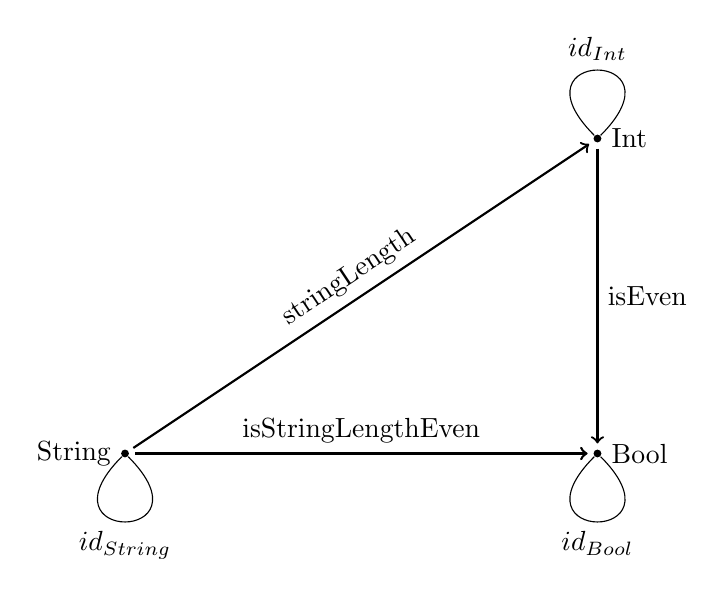
\begin{tikzpicture}[ele/.style={fill=black,circle,minimum
        width=.8pt,inner sep=1pt},every fit/.style={ellipse,draw,inner
        sep=-2pt}]
    % the texts    
    \node[ele,label=right:Int] (int) at (6,4) {};    
    \node[ele,label=right:Bool] (bool) at (6,0) {};    
    \node[ele,label=left:String] (string) at (0,0) {};

    \draw[->,thick,shorten <=2pt,shorten >=2pt] (int) to
    node[right]{isEven} (bool); 
    \draw[->,thick,shorten <=2pt,shorten >=2] (string) to
    node[pos=0.5,sloped,above]{stringLength} (int); 
    \draw[->,thick,shorten <=2pt,shorten >=2] (string) to
    node[pos=0.5,sloped,above]{isStringLengthEven} (bool); 
    \draw[->,thick,shorten <=2pt,shorten >=2] (string) -- (bool);
    \draw (int) to [out=45,in=135,looseness=50] node[above]
          {$id_{Int}$} (int); 
    \draw (string) to [out=-45,in=-135,looseness=50] node[below]
          {$id_{String}$} (string); 
    \draw (bool) to [out=-45,in=-135,looseness=50] node[below]
          {$id_{Bool}$} (bool); 

  \end{tikzpicture}
  \caption{Programming language category example. Objects are types: Int,
    Bool, String. Morphisms are several functions}
  \label{fig:pl_example}
\end{figure}


\subsubsection{\textbf{Hask} category}
\begin{example}[\textbf{Hask} category]
  \label{ex:haskcategory}
  \index{Object!\textbf{Hask} example}
  \index{Morphism!\textbf{Hask} example}
  Types in Haskell are considered as \mynameref{def:object}s.
  Functions are considered as \mynameref{def:morphism}s.
  We are going to implement \mynameref{def:category} from
  \cref{fig:pl_example}.

  The function isEven that converts Int type
  into Bool.
  \begin{minted}{haskell}
    isEven :: Int -> Bool
    isEven x = x `mod` 2 == 0
  \end{minted}

  There is also \mynameref{def:id} that is defined as follows
  \begin{minted}{haskell}
    id :: a -> a
    id x = x
  \end{minted}

  If we have an additional function
  \begin{minted}{haskell}
    stringLength :: String -> Int
    stringLength x = length x
  \end{minted}
  then we can create a \mynameref{prop:composition}
  \begin{minted}{haskell}
    isStringLengthEven :: String -> Bool
    isStringLengthEven = isEven . stringLength
  \end{minted}

  %% If we consider pure (without effects) functions then
  %% \mynameref{prop:associativity} is also satisfied.
\end{example}

%http://math.andrej.com/2016/08/06/hask-is-not-a-category/
\begin{remark}[Haskell lazy evaluation]
  Each Haskell type has a special value $\bot$. The value presents
  and lazy evaluations make several category law invalid, for instance
  \mynameref{def:id} behaviour become invalid in specific cases:

  The following code
  \begin{minted}{haskell}
    seq undefined True
  \end{minted}
  produces \textit{undefined}
  But the following
  \begin{minted}{haskell}
    seq (id.undefined) True
    seq (undefined.id) True
  \end{minted}
  produces \textit{True} in both cases.
  As result we have
  (we cannot compare compare functions in Haskell, but if we
  could we can get the following)
  \begin{minted}{haskell}
    id . undefined /= undefined
    undefined . id /= undefined,
  \end{minted}
  i.e. \eqref{eq:leftid} and
  \eqref{eq:rightid} are not satisfied.  
\end{remark}

\subsubsection{\textbf{C++} category}
\begin{example}[\textbf{C++} category]
  \label{ex:cppcategory}
  \index{Object!\textbf{C++} example}
  \index{Morphism!\textbf{C++} example}
  We will use the same trick as in \mynameref{ex:haskcategory} and
  will assume 
  types in C++ as \mynameref{def:object}s, 
  functions as \mynameref{def:morphism}s.
  We also are going to implement
  \mynameref{def:category} from \cref{fig:pl_example}.


  We  also define 2 functions:
  \begin{minted}{c++}
    auto isEven = [](int x) { 
      return x % 2 == 0; 
    };

    auto stringLength = [](std::string s) { 
      return static_cast<int>(s.size()); 
    };
  \end{minted}

  Composition can be defined as follows:
  \begin{minted}{c++}
    // h = g . f
    template <typename A, typename B> 
    auto compose(A g, B f) {
      auto h = [f, g](auto a) {
        auto b = f(a);
        auto c = g(b);
        return c;
      };
      return h;
    };
  \end{minted}

  The \mynameref{def:id}:
  \begin{minted}{c++}
    auto id = [](auto x) { return x; };
  \end{minted}

  The usage examples are the following:
  \begin{minted}{c++}
    auto isStringLengthEven = compose<>(isEven, stringLength);

    auto isStringLengthEvenL = compose<>(id, isStringLengthEven);

    auto isStringLengthEvenR = compose<>(isStringLengthEven, id);  
  \end{minted}

  Such construction will always provides us the category as soon as we
  use pure function (functions without effects).
\end{example}
